\documentclass[tikz,border=7pt]{standalone}
\usepackage[T1]{fontenc}
\usepackage{lmodern,amsmath,amssymb}
\usetikzlibrary{arrows.meta,calc,positioning,backgrounds,fit}
\definecolor{ink}{HTML}{1E293B}
\definecolor{blue}{HTML}{2563EB}
\definecolor{teal}{HTML}{0F766E}
\definecolor{orange}{HTML}{B45309}
\definecolor{purple}{HTML}{6D28D9}
\begin{document}
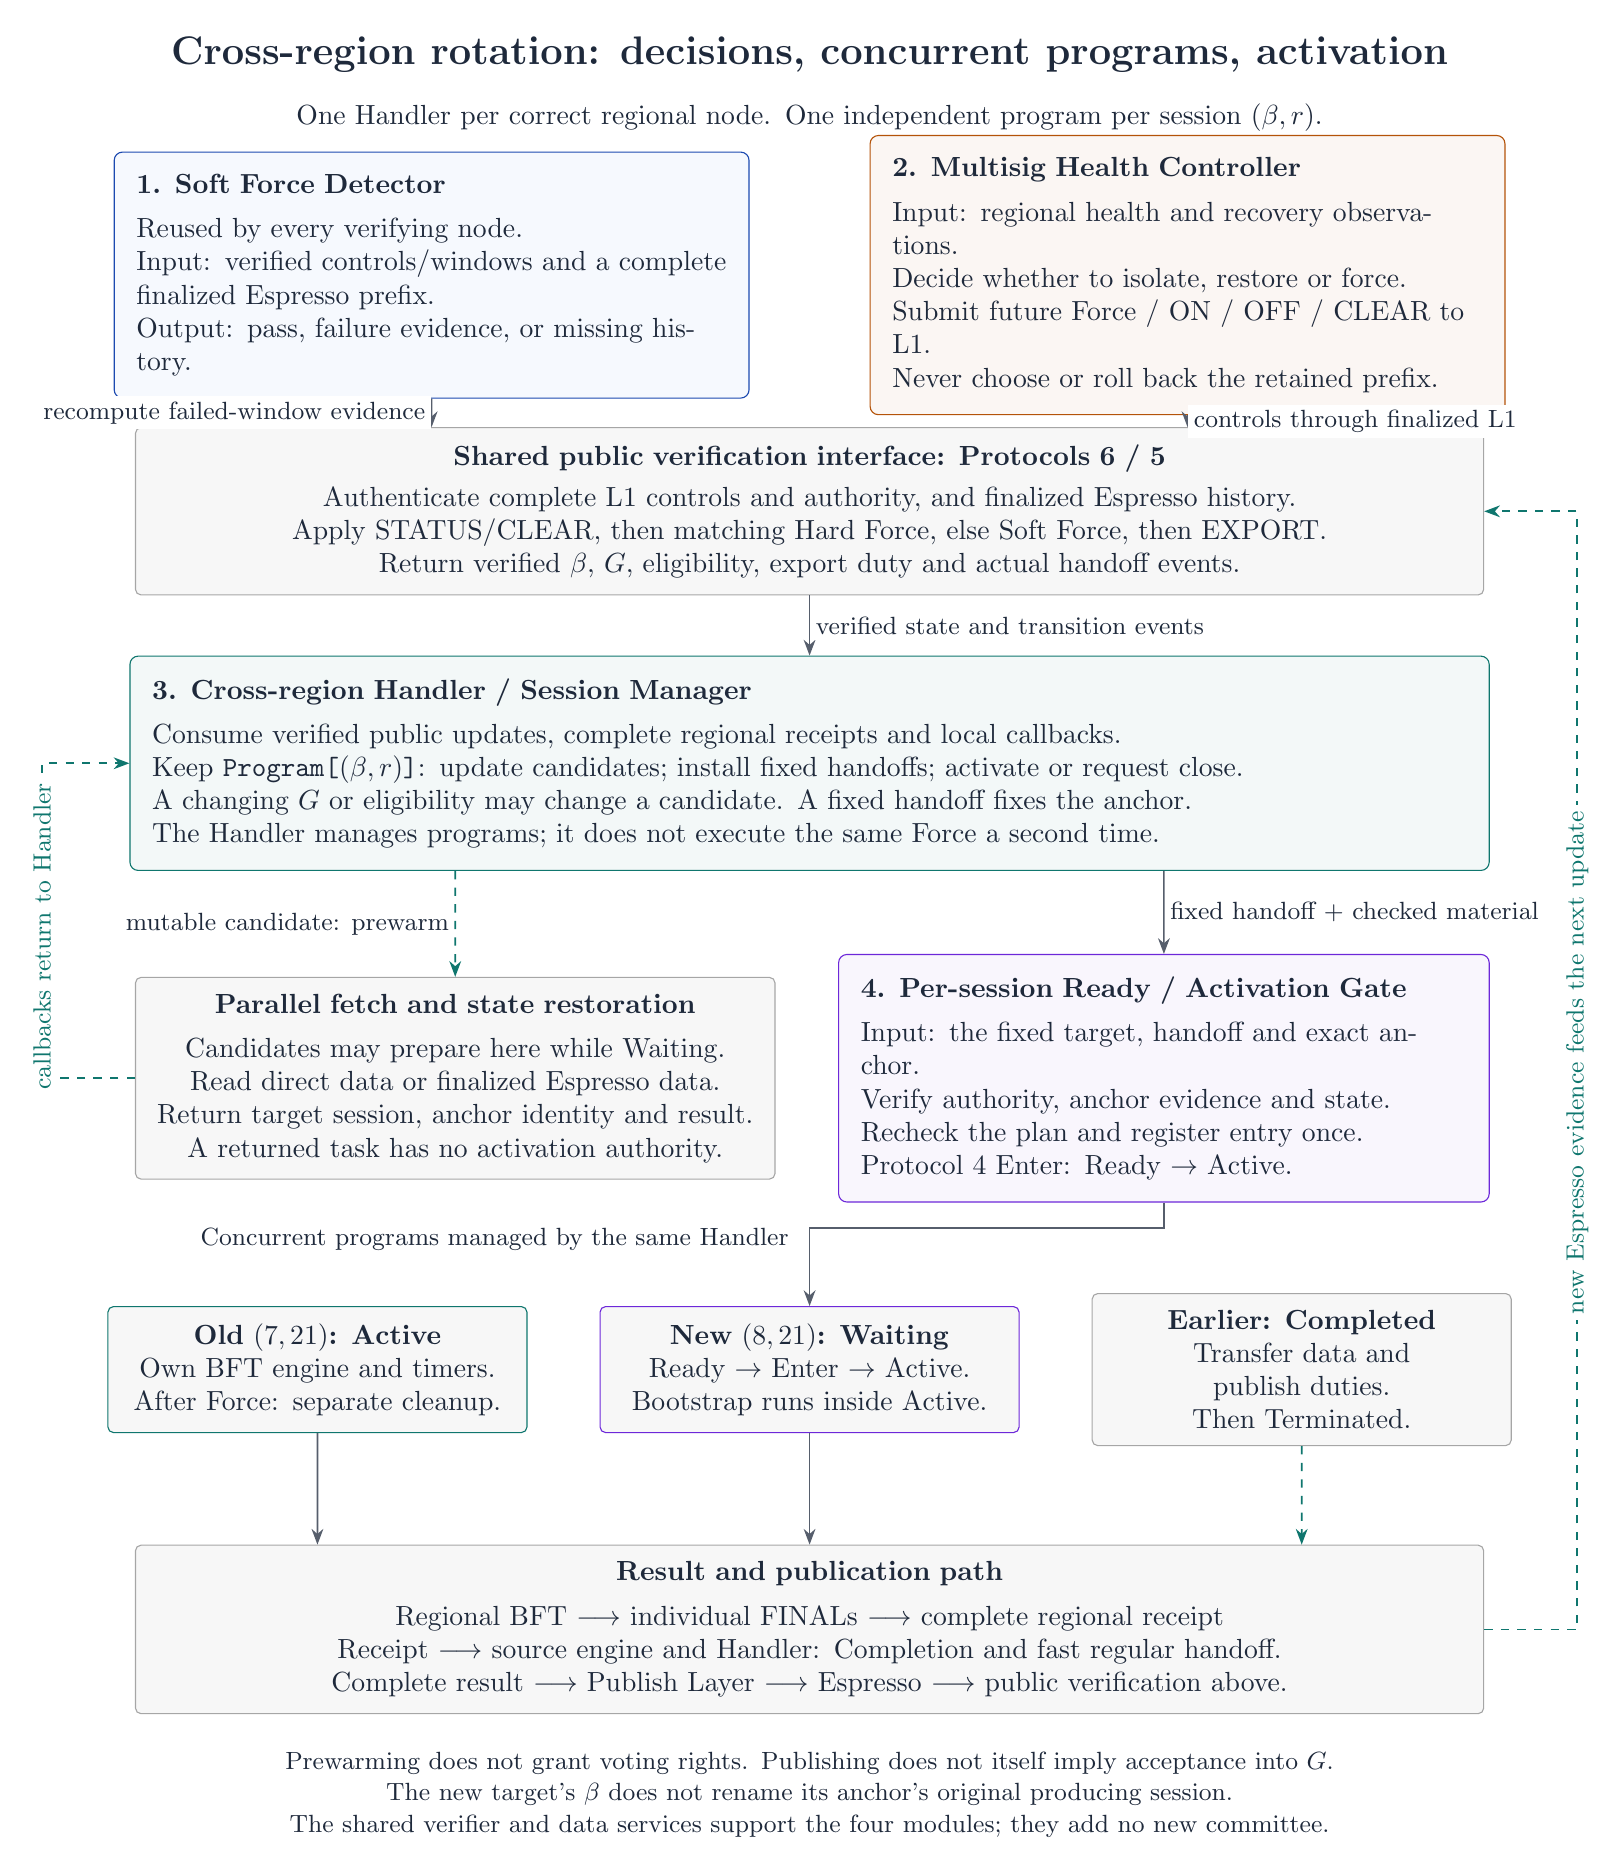
\begin{tikzpicture}[
 x=1cm,y=-1cm,font=\fontsize{10}{12}\selectfont,text=ink,
 source/.style={draw=black!35,fill=black!3,rounded corners=2pt,align=center,inner sep=6pt},
 module/.style={draw=blue!75!black,fill=blue!4,rounded corners=3pt,align=left,inner sep=8pt},
 flow/.style={-{Stealth[length=2mm]},semithick,draw=ink!75},
 async/.style={flow,dashed,draw=teal},
 lab/.style={fill=white,inner sep=2pt,font=\fontsize{8.8}{10.5}\selectfont,align=center}
]
\node[font=\fontsize{15}{18}\selectfont\bfseries,align=center] at (9,0)
 {Cross-region rotation: decisions, concurrent programs, activation};
\node[align=center,text width=18cm] at (9,.8)
 {One Handler per correct regional node. One independent program per session $(\beta,r)$.};
\node[module,text width=7.5cm,minimum height=2.65cm] (soft) at (4.2,2.8)
 {\textbf{1. Soft Force Detector}\\[4pt]
 Reused by every verifying node.\\
 Input: verified controls/windows and a complete\\finalized Espresso prefix.\\
 Output: pass, failure evidence, or missing history.};
\node[module,draw=orange,fill=orange!5,text width=7.5cm,minimum height=2.65cm] (hard) at (13.8,2.8)
 {\textbf{2. Multisig Health Controller}\\[4pt]
 Input: regional health and recovery observations.\\
 Decide whether to isolate, restore or force.\\
 Submit future Force / ON / OFF / CLEAR to L1.\\
 Never choose or roll back the retained prefix.};
\node[source,text width=16.7cm,minimum height=1.8cm] (verify) at (9,5.8)
 {\textbf{Shared public verification interface: Protocols 6 / 5}\\[3pt]
 Authenticate complete L1 controls and authority, and finalized Espresso history.\\
 Apply STATUS/CLEAR, then matching Hard Force, else Soft Force, then EXPORT.\\
 Return verified $\beta$, $G$, eligibility, export duty and actual handoff events.};
\draw[flow] (soft.south)--node[lab,left] {recompute failed-window evidence} ([xshift=-4.8cm]verify.north);
\draw[flow] (hard.south)--node[lab,right] {controls through finalized L1} ([xshift=4.8cm]verify.north);
\node[module,draw=teal,fill=teal!5,text width=16.7cm,minimum height=2.35cm] (manager) at (9,9.0)
 {\textbf{3. Cross-region Handler / Session Manager}\\[4pt]
 Consume verified public updates, complete regional receipts and local callbacks.\\
 Keep \texttt{Program[}$(\beta,r)$\texttt{]}: update candidates; install fixed handoffs; activate or request close.\\
 A changing $G$ or eligibility may change a candidate. A fixed handoff fixes the anchor.\\
 The Handler manages programs; it does not execute the same Force a second time.};
\draw[flow] (verify.south)--node[lab,right] {verified state and transition events}(manager.north);
\node[module,draw=purple,fill=purple!4,text width=7.7cm,minimum height=2.55cm] (gate) at (13.5,13.0)
 {\textbf{4. Per-session Ready / Activation Gate}\\[4pt]
 Input: the fixed target, handoff and exact anchor.\\
 Verify authority, anchor evidence and state.\\
 Recheck the plan and register entry once.\\
 Protocol 4 Enter: Ready $\to$ Active.};
\node[source,text width=7.7cm,minimum height=2.55cm] (fetch) at (4.5,13.0)
 {\textbf{Parallel fetch and state restoration}\\[4pt]
 Candidates may prepare here while Waiting.\\
 Read direct data or finalized Espresso data.\\
 Return target session, anchor identity and result.\\
 A returned task has no activation authority.};
\draw[async] ([xshift=-4.5cm]manager.south)--node[lab,left] {mutable candidate: prewarm}(fetch.north);
\draw[flow] ([xshift=4.5cm]manager.south)--node[lab,right] {fixed handoff + checked material}(gate.north);
\draw[async] (fetch.west)--(-.75,13)--(-.75,9)--(manager.west);
\node[lab,rotate=90,text=teal] at (-.75,11.2) {callbacks return to Handler};
\node[source,draw=teal,text width=4.9cm,minimum height=1.6cm] (old) at (2.75,16.7)
 {\textbf{Old $(7,21)$: Active}\\Own BFT engine and timers.\\After Force: separate cleanup.};
\node[source,draw=purple,text width=4.9cm,minimum height=1.6cm] (new) at (9,16.7)
 {\textbf{New $(8,21)$: Waiting}\\Ready $\to$ Enter $\to$ Active.\\Bootstrap runs inside Active.};
\node[source,text width=4.9cm,minimum height=1.6cm] (done) at (15.25,16.7)
 {\textbf{Earlier: Completed}\\Transfer data and publish duties.\\Then Terminated.};
\draw[flow] (gate.south)--(13.5,14.9)--(9,14.9)--(new.north);
\node[lab] at (5,15.05) {Concurrent programs managed by the same Handler};
\node[source,text width=16.7cm,minimum height=1.8cm] (results) at (9,20.0)
 {\textbf{Result and publication path}\\[4pt]
 Regional BFT $\longrightarrow$ individual FINALs $\longrightarrow$ complete regional receipt\\
 Receipt $\longrightarrow$ source engine and Handler: Completion and fast regular handoff.\\
 Complete result $\longrightarrow$ Publish Layer $\longrightarrow$ Espresso $\longrightarrow$ public verification above.};
\draw[flow] (old.south)--(2.75,18.4)--([xshift=-6.25cm]results.north);
\draw[flow] (new.south)--(results.north);
\draw[async] (done.south)--(15.25,18.4)--([xshift=6.25cm]results.north);
\draw[async] (results.east)--(18.75,20)--(18.75,5.8)--(verify.east);
\node[lab,rotate=90,text=teal] at (18.75,12.8) {new Espresso evidence feeds the next update};
\node[align=center,text width=18cm,font=\fontsize{9.5}{11.5}\selectfont] at (9,22.1)
 {Prewarming does not grant voting rights. Publishing does not itself imply acceptance into $G$.\\
 The new target's $\beta$ does not rename its anchor's original producing session.\\
 The shared verifier and data services support the four modules; they add no new committee.};
\end{tikzpicture}
\end{document}
